\chapter{Re-weighting of the $W/Z$ boson $\pt$}
    \label{app:BosonPtReweight}

The comparison of the boson $\pt$ distribution in the control regions, in data and simulation, indicates that the Monte Carlo overestimates the tail of the measured distribution.
This is attributed to an inadequate modeling of the true boson $\pt$ that recoils the rest of the hadronic final state.
Therefore, a re-weighting procedure is applied to correct the generated boson $\pt$ distribution in the MC.

Weights are determined separately for $\wen$+jets, $\wmn$+jets and $\zmm$+jets control regions, and found to be compatible.
Nonetheless, the weights obtained from the $\wmn$+jets control region are adopted due to its higher statistical power.
These weights are shown in Figure \ref{fig:BosonPtWeights}.
The statistics in the region $\pt^{\text{boson}} > \unit[400]{GeV}$ is limited, and a single weight is therefore employed to correct the modeling of the boson $\pt$ in these events.

\begin{figure}[!ht]
  \begin{center}
    \mbox{
      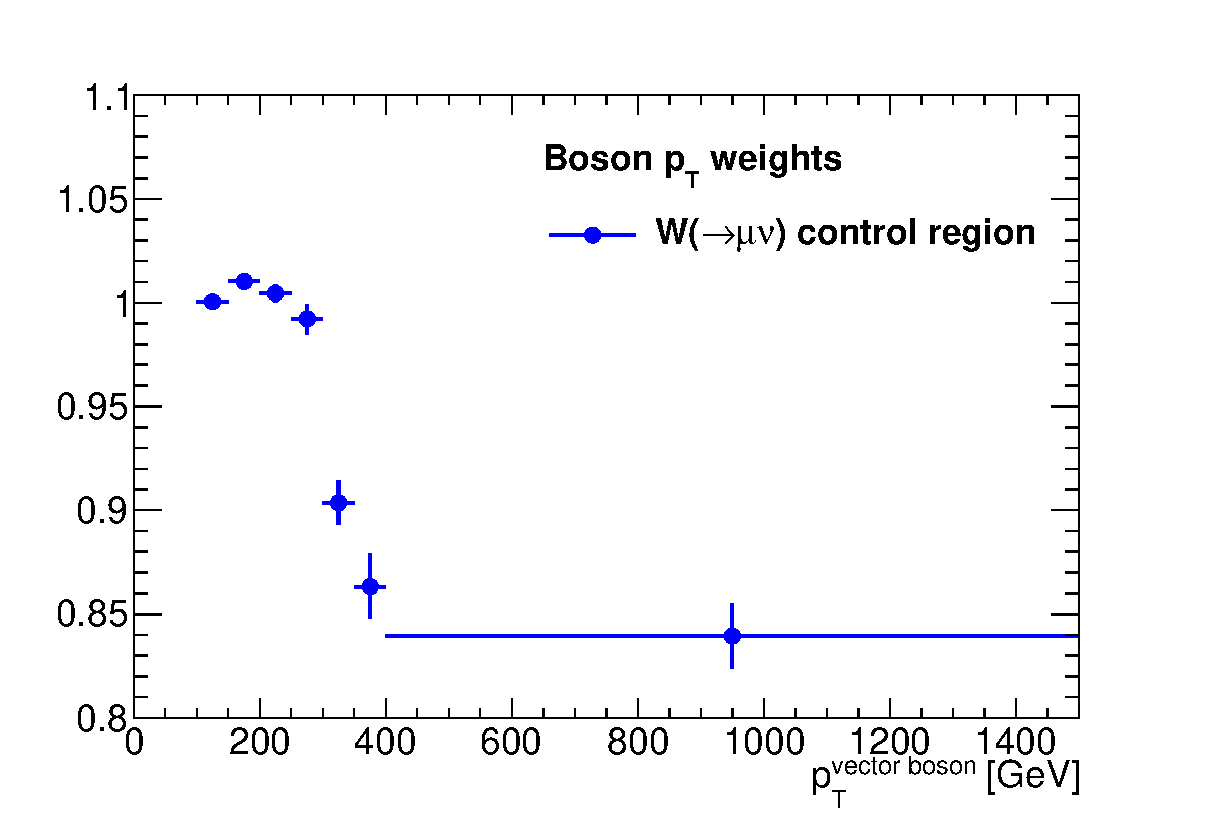
\includegraphics[width=0.635\textwidth]{Appendix_BosonPtReweight/Figures/BosonPtWeights.eps}
    }
  \end{center}
  \caption{Weights applied to the generated boson $\pt$ in the $W/Z$+jets MC samples.}
  \label{fig:BosonPtWeights}
\end{figure}

Figure~\ref{fig:bosonptwcheck} shows the impact of the $\pt$ re-weighting in the boson $\pt$ and the $\met$ distributions for the signal region M1.
The distributions in this figure do not include the multijet contribution and only show the statistical uncertainties, but they remain sufficient to validate the re-weighting.
As expected, the shape of the distribution is adjusted to that of the data.

\begin{figure}
\begin{center}
\mbox{
  \includegraphics[width=0.49\textwidth]{Appendix_BosonPtReweight/Figures/plot_Stop_A6_SR_bosonVec_reco_pt_fitted_NoBosonPtReweight.eps}
  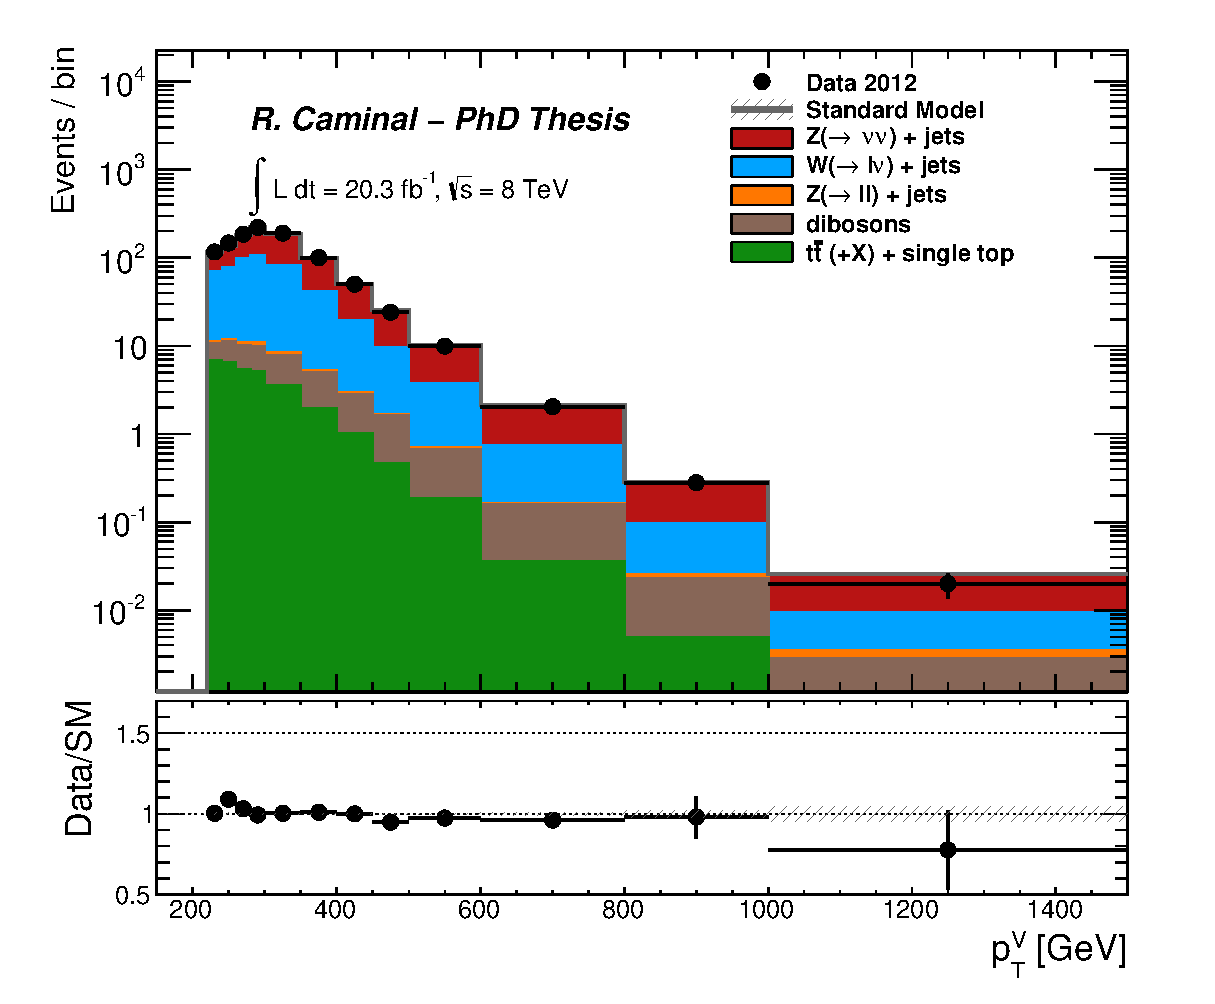
\includegraphics[width=0.49\textwidth]{Appendix_BosonPtReweight/Figures/plot_Stop_A6_SR_bosonVec_reco_pt_fitted_BosonPtReweightApplied.eps}
}
\mbox{
  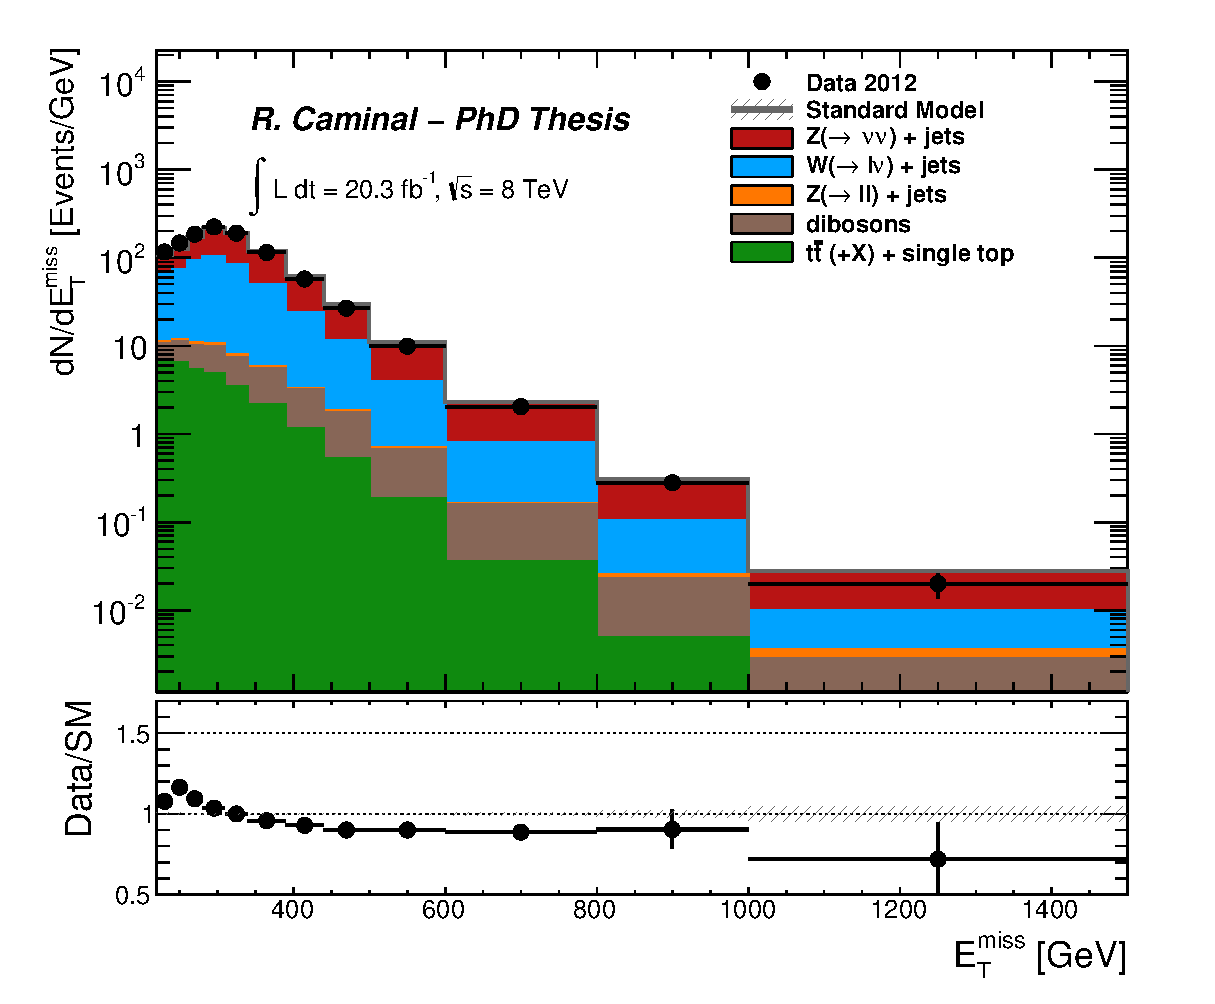
\includegraphics[width=0.49\textwidth]{Appendix_BosonPtReweight/Figures/plot_Stop_A6_SR_met_fitted_NoBosonPtReweight.eps}
  \includegraphics[width=0.49\textwidth]{Appendix_BosonPtReweight/Figures/plot_Stop_A6_SR_met_fitted_BosonPtReweightApplied.eps}
}
\end{center}
\caption[Distributions for the boson $\pt$ and the $\met$ in the signal region M1.]{
Distributions for the boson $\pt$ (top) and the $\met$ (bottom) in the signal region M1. The distributions on the left do not include the boson $\pt$ re-weighting, whereas the distributions on the right do so. Only the statistical uncertainties are shown in the distributions.}
\label{fig:bosonptwcheck}
\end{figure}
